\documentclass[11pt,a4paper]{article}
\usepackage[utf8]{inputenc}
\usepackage[T1]{fontenc}
\usepackage{amsmath}
\usepackage{amssymb}
\usepackage{subcaption}
\usepackage{float}
\usepackage{graphicx}
\usepackage{enumerate}
\usepackage{hyperref}
\usepackage{amsthm}
\newcommand{\y}{\mathrm{y}}
\newcommand{\x}{\mathrm{x}}
\newcommand{\z}{\mathrm{z}}
\newcommand{\R}{\mathbb{R}}
%\graphicspath{ {} }
\usepackage[left=2.00cm, right=2.00cm, top=2.00cm, bottom=2.00cm]{geometry}

\begin{document}
	\begin{figure}
		\centering
		\includegraphics[scale = 0.1]{C:/Users/hp/OneDrive - LUT University/Bureau/LUT logo}
		%\caption{Caption}
		%\label{fig:my_label}
	\end{figure}
	%%%%%%%%%%%%%%%%%%%%%%% title page %%%%%%%%%%%%%%%%%%%%%%%%%%
	\thispagestyle{empty}
	\begin{center}
		\textbf{\\[0.5cm]
		}
		\vspace{0.01cm}
	\end{center}
	
	%%%%%%%%%%%%%%%%%%%%% assignment information %%%%%%%%%%%%%%%%
	\noindent
	\rule{17cm}{0.2cm}\\[0.3cm]
	Name: Kamdem Louis Mozart \hfill Homework 1\\[0.1cm]
	Course:Statistical Parameter Estimation \hfill Date: \today\\
	\rule{17cm}{0.05cm}
	\vspace{1.0cm}
	\begin{align*}
		y(t) = a\exp(-bt)+\epsilon(t),\quad \epsilon(t)\sim\mathcal{N}(0,\sigma^{2})
	\end{align*}
with $ \sigma = 0.02 $. \\
Original simulation values are $ a = 0.4 $ and $ b = 3 $. We denote $ \theta := (a, b)^{T} $

\begin{enumerate}
\item Likelihood density.
   \begin{itemize}
     	\item Write the likelihood of $ \theta $ given $ y(t) $\\\\
     	We have from the Bayes formula:
     	\begin{align*}
     		p(\theta|y(t)) = \frac{p\big(y(t)|\theta\big)p(\theta)}{p\big(y(t)\big)}\propto p\big(y(t)|\theta\big)p(\theta)
     	\end{align*}
     The likelihood is:\begin{align*}
     	\mathcal{L}(\theta) = p\big(y(t)|\theta\big) = \prod_{i=1}^{n} p\big(y({t_i})|\theta\big) = \prod_{i=1}^{n} \frac{1}{\sqrt{2\pi\sigma^{2}}}e^{-1/2\big(\frac{y(t_i)-ae^{-bt_i}}{\sigma}\big)^{2}} 
     \end{align*}
 So the likelihood is, \begin{align*}
 	\boxed{	\mathcal{L}(\theta)  = \bigg(\frac{1}{2\pi\sigma^{2}}\bigg)^{n/2}\exp\bigg({-\frac{1}{2\sigma^{2}}\sum_{i=1}^{n}\big(y(t_i)-ae^{-bt_i}\big)^{2}}\bigg)}
 \end{align*}
\item The negative log likelihood\\\\
The negative log likelihood $ \ell(\theta)$ of $ \theta $ is given by: \begin{align*}
	 &= -\log(\mathcal{L}(\theta))\\
	& = -\log\bigg(\bigg(\frac{1}{2\pi\sigma^{2}}\bigg)^{n/2}\exp\bigg({-\frac{1}{2\sigma^{2}}\sum_{i=1}^{n}\big(y(t_i)-ae^{-bt_i}\big)^{2}}\bigg) \bigg)\\
	& = \frac{n}{2}\log(2\pi\sigma^{2})+\frac{1}{2\sigma^{2}}\sum_{i=1}^{n}\big(y(t_i)-ae^{-bt_i}\big)^{2}
\end{align*} 
So, the negative log likelihood is:
\begin{align*}
	\boxed{\ell(\theta) = \frac{n}{2}\log(2\pi\sigma^{2})+\frac{1}{2\sigma^{2}}\sum_{i=1}^{n}\big(y(t_i)-ae^{-bt_i}\big)^{2}}
\end{align*}
   \end{itemize}
\item Optimization:\\\\ The maximum likelihood estimates $ \hat{\theta}_{ML} $ is obtained by maximizing the likelihood or equivantly by minimizing the negative log likelihood. i.e:
\begin{align*}
	\boxed{\hat{\theta}_{ML} = \underset{\theta}{\text{argmin }}\ell(\theta)=\underset{a,b}{\text{argmin }}\dfrac{n}{2}\log(2\pi\sigma^{2}) + \dfrac{1}{2\sigma^{2}}\sum_{i=1}^{n}\big(y(t_i)-ae^{-bt_i}\big)^{2}}
\end{align*}
\item Priors and integrations
\begin{itemize}
	\item Choose a Gaussian prior for $ \theta $ and define a posterior distribution.
	Calculate the negative log posterior. Calculate the MAP and CM estimators.\\\\
	
	The conditionnal mean estimator is defined by: \begin{align*}
		\hat{\theta}_{CM} = \mathbb{E}(\theta|y) = \int_{\R^2}\theta p(\theta|y)d\theta
	\end{align*}
But we know that the posterior is define as: \begin{align*}
	 p(\theta|y)& \propto p(\theta)\mathcal{L}(\theta)\\
	 & = p(\theta)\frac{1}{\sqrt{(2\pi)^n\lvert \sigma^2I\rvert}}\exp\big(-\frac{1}{2\sigma^2}\lVert y-f(t,\theta)\rVert_2^2\big)
\end{align*}
where $ \lVert y-f(t,\theta)\rVert_2^2 = \sum_{i=1}^{n}\big(y(t_i)-f(t_i,\theta)\big)^{2} $ with $ f(t_i,\theta) = ae^{-bt_i} $\\
By choosing a gaussian distributed prior with mean $ \mu $ and variance matrix $ \Sigma $, i.e.\begin{align*}
	p(\theta) = \sqrt{\frac{1}{(2\pi)^2\lvert\Sigma\rvert} }\exp\big(-\dfrac{1}{2}(\theta-\mu)^{T}\Sigma^{-1}(\theta-\mu)\big)
\end{align*}
Putting everything back into the conditional mean estimator formula yield
\begin{align*}
	\boxed{\hat{\theta}_{CM} =  \sqrt{\frac{1}{(2\pi)^{n+2}\lvert\Sigma\rvert\lvert\sigma^2I\rvert} }\int_{\R^2}\theta\exp\bigg(-\dfrac{1}{2}(\theta-\mu)^{T}\Sigma^{-1}(\theta-\mu)-\frac{1}{2\sigma^2}\lVert y-f(t,\theta)\rVert_2^2\bigg)d\theta}
\end{align*}
The MAP estimator is obtained by minimizing the negative log posterior.\\
The negative log posterior is 
\begin{align*}
	\ell_{p}(\theta) &= -\log\big(p(\theta|y)\big)\\
	& =-\log\big(p(\theta)\big)+\dfrac{n}{2}\log(2\pi)+ \dfrac{1}{2}\log(\lvert \sigma^{2}I\rvert)  + \frac{1}{2\sigma^2}\lVert y-f(t,\theta)\rVert_2^2
\end{align*}
With the choosen prior, the MAP estimator is then given by  \\
\begin{align*}
	\boxed{\hat{\theta}_{MAP} = \underset{\theta}{argmin }\quad C+\frac{1}{2}(\theta-\mu)^{T}\Sigma^{-1}(\theta-\mu)+ \frac{1}{2\sigma^2}\lVert y-f(t,\theta)\rVert_2^2}
\end{align*}
Where $ C $ is a constant.
\item  Do the same as above, but choose a prior distribution that is
uniformly distributed.\\
Let's consider a uniform distributed prior with parameters $ c_0 $ and $ c_1 $ i.e. \begin{align*}
	p(\theta)  = \begin{cases}
		1\quad \text{if } a,b\in [c_0,c_1]\\
		0\quad \text{else}
	\end{cases}
\end{align*} 
ACcording to these parameters, the CM and MAP estimate becomes:
\begin{align*}
		\boxed{\hat{\theta}_{CM} =  \frac{1}{\sqrt{(2\pi)^n\lvert \sigma^2I\rvert}}\int_{c_0}^{c_1}\int_{c_0}^{c_1}\theta\exp\big(-\frac{1}{2\sigma^2}\lVert y-f(t,\theta)\rVert_2^2\big)d\theta}
\end{align*}
and,
\begin{align}\label{1}
	\boxed{\hat{\theta}_{MAP} = \underset{\theta}{argmin} -\log(p(\theta))+\log(\lvert \sigma^{2}I\rvert)+(\frac{n}{2})\log(2\pi)+ \frac{1}{2\sigma^2}\lVert y-f(t,\theta)\rVert_2^2}
\end{align}
\item Marginal densities of $ a $ and $ b $:\\
The marginal densities here  are computed py using only the prior Gaussian distribution so $ p(\theta)\sim \mathcal{N}(\mu,\Sigma) $.
Therefore,\begin{align*}
	p(a) = \frac{1}{\sqrt{(2\pi)^2\lvert\Sigma\rvert}}\int_{\R}\exp\big(-\frac{1}{2}(\theta-\mu)^T\Sigma^{-1}(\theta-\mu)\big)db\\
	p(b) = \frac{1}{\sqrt{(2\pi)^2\lvert\Sigma\rvert}}\int_{\R}\exp\big(-\frac{1}{2}(\theta-\mu)^T\Sigma^{-1}(\theta-\mu)\big)da
\end{align*}
 
\end{itemize}
\item Visualizations
\begin{itemize}
	\item Plot data and ground truth in the same plot.
\begin{figure}[H]
	\centering
	\begin{subfigure}{0.49\textwidth}
		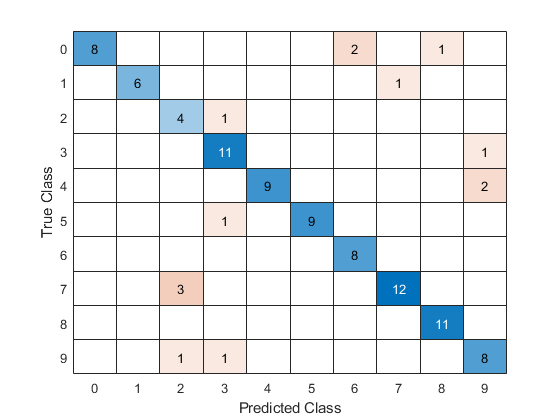
\includegraphics[width=\textwidth]{fig1}
		\caption{Data}
		\label{fig4:first}
	\end{subfigure}
	\begin{subfigure}{0.49\textwidth}
		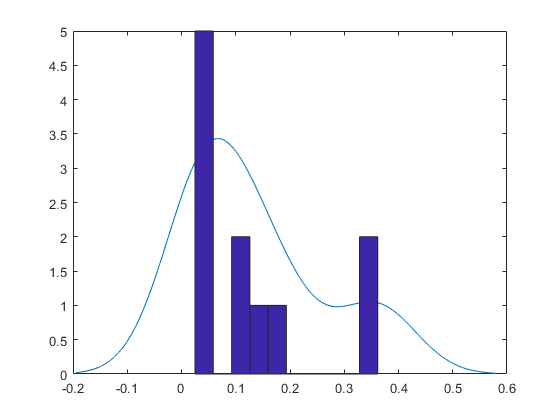
\includegraphics[width=\textwidth]{fig2}
		\caption{Data distribution}
		\label{fig4:first}
	\end{subfigure}
\caption{Data and groundthruth}
\end{figure}
\item Take all the parameter estimates calculated above and plot the corresponding curves. 

\begin{figure}[H]
	\centering
	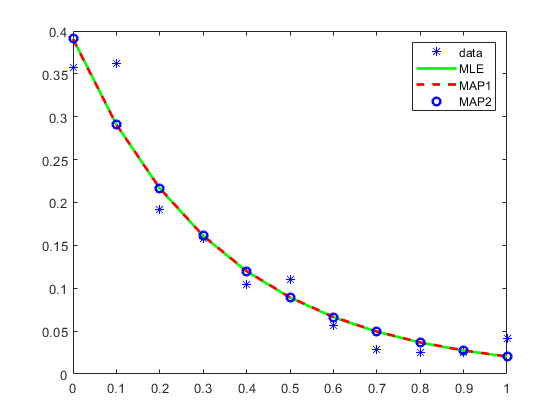
\includegraphics[width=0.5\textwidth]{fig3}
	\caption{curves for each estimator}
	\label{FIG2:first}
\end{figure}
In the figure (\ref{FIG2:first}) above, with a gaussian prior of parameters $ \mu = 0 $ and variance $ \Sigma = \sigma^2 I$ and a uniform prior of parameter 0, 1 we can see how they all coincide with the MLE extimator.
\item marginal density of $ a $ and $ b $\\
We choosed a gaussian prior distribution for $ \theta $ to get the marginal density of $ a $ and $ b $. The parameters are $ \mu = [0 \quad2] $ and $ \Sigma = \begin{pmatrix}
	4&0\\
	0&4
\end{pmatrix} $. The implementation gives:
\begin{figure}[H]
	\centering
	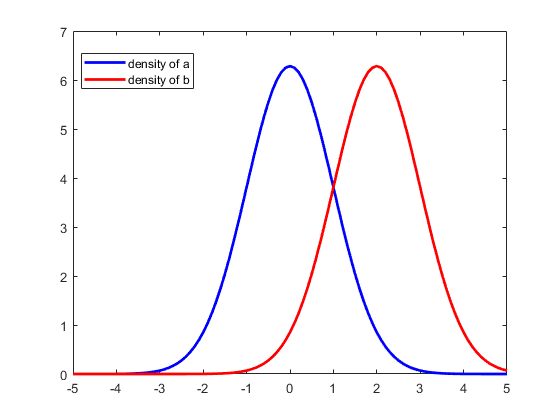
\includegraphics[width=0.5\textwidth]{fig4}
	\caption{Marginal density of the parameter with a gaussian prior }
	\label{FIG4:first}
\end{figure}
\item Tune the prior parameters and study how the parameter values affect the estimators and curves.\\

We already found in figure (\ref{FIG2:first}) that the MAP estimator with the Uniform prior of parameter 0, 1 and the gaussian prior with parameter $ \mu = [0\quad 0] $ and $ \Sigma = \sigma^2I $ coincide with the MLE estimator. During the whole experience, we found that the MLE estimator always coincide with the MAP estimator when the prior is uniformly distributed no matter what are the parameters. This can be explained by the fact in the additionnal the first term of the MAP estimator in equation (\ref{1}) will be equal to zero if the prior is uniform and we only remain with the same function to minimize as in the case of the likelihood. So, we will only tuned the parameters of the Gaussian prior in this report. First we fixed the variance at $ \Sigma = \sigma^2 I $ and we played with different values of the mean. Here are the result.
\begin{figure}[H]
	\centering
	\begin{subfigure}{0.4\textwidth}
		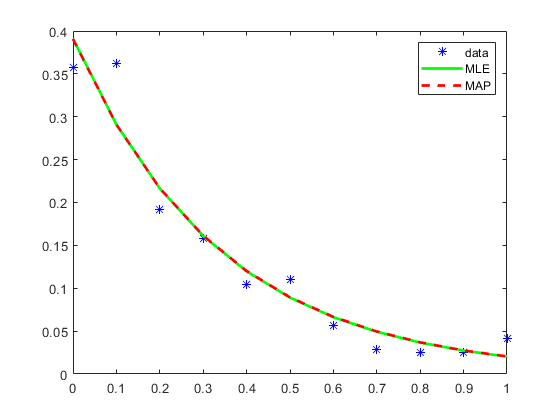
\includegraphics[width=\textwidth]{fig5}
			\caption{$ \mu  = [0\quad0]$}
		\label{fig4:first}
	\end{subfigure}
	\begin{subfigure}{0.4\textwidth}
		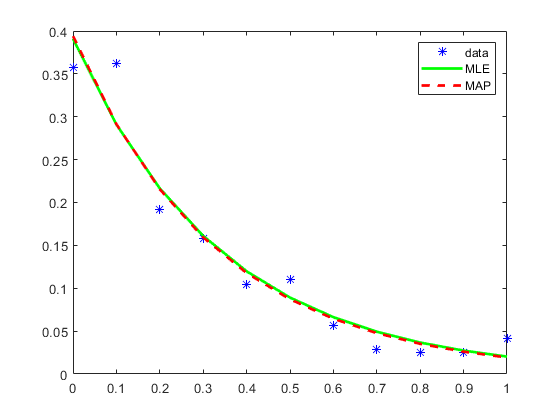
\includegraphics[width=\textwidth]{fig6}
			\caption{$ \mu  = [10\quad20]$}
		\label{fig4:first}
	\end{subfigure}
	\begin{subfigure}{0.4\textwidth}
		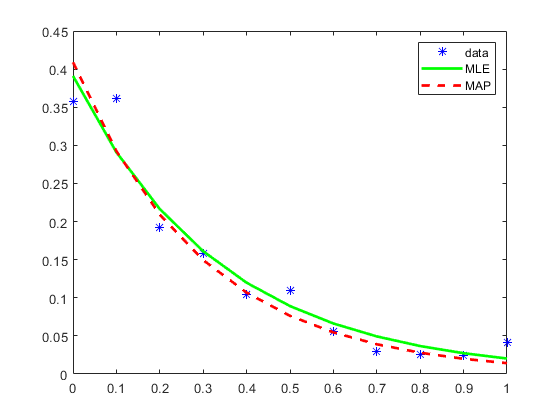
\includegraphics[width=\textwidth]{fig7}
		\caption{$ \mu  = [50\quad100]$}
		\label{fig4:first}
	\end{subfigure}
	\begin{subfigure}{0.4\textwidth}
		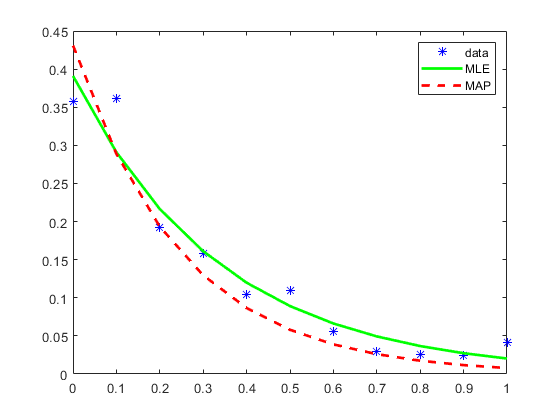
\includegraphics[width=\textwidth]{fig8}
			\caption{$ \mu  = [100\quad200]$}
		\label{fig4:first}
	\end{subfigure}
\end{figure}
Secondly, we fixed the mean as $ \mu =[0\quad 0] $ and we use the variance of the form $ \Sigma = \sigma^2 I $ were we played with different values of $ \sigma $ to see what happened.
\begin{figure}[H]
	\centering
	\begin{subfigure}{0.4\textwidth}
		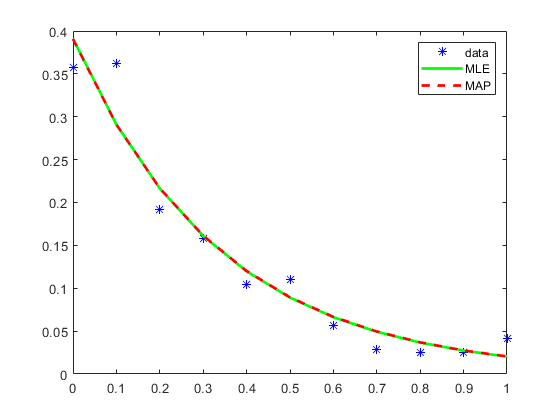
\includegraphics[width=\textwidth]{fig9}
		\caption{$ \sigma  = 0.02$}
		\label{fig4:first}
	\end{subfigure}
	\begin{subfigure}{0.4\textwidth}
		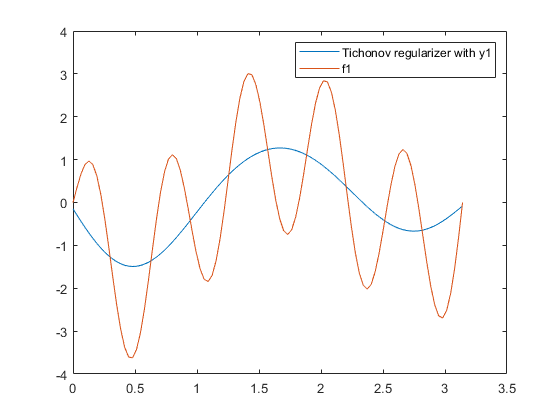
\includegraphics[width=\textwidth]{fig10}
		\caption{$ \sigma  = 0.1$}
		\label{fig4:first}
	\end{subfigure}
	\begin{subfigure}{0.4\textwidth}
		\includegraphics[width=\textwidth]{fig11}
		\caption{$\sigma  = 0.25$}
		\label{fig4:first}
	\end{subfigure}
	\begin{subfigure}{0.4\textwidth}
		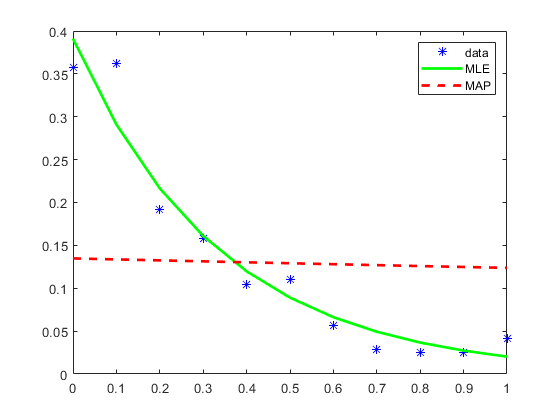
\includegraphics[width=\textwidth]{fig12}
		\caption{$ \sigma  = 0.5$}
		\label{fig4:first}
	\end{subfigure}
\end{figure}
\end{itemize}
The graphs shows that the prior is more sensitive to the variance matrix than to the mean and a small change in the variance matrix rise to a big change on the MAP estimator. 
\end{enumerate}

\end{document}